\section{\it Max 2D Range Sum}

\begin{frame}[fragile]{Definição}

    \metroset{block=fill}
    \begin{block}{Max 2D Range Sum}
        Seja $A$ uma matriz $n \times m$. O \textit{max 2D range sum} da matriz $A$ é a submatriz
            $B_{r\times s}$ de $A$ cuja soma
        \[
            \sum_{i = 1}^r \sum_{j = 1}^s b_{ij}
        \]
        é máxima.
    \end{block}

\end{frame}

\begin{frame}[fragile]{Características do {\it Max 2D Range Sum}}

    \begin{itemize}
        \item Assim como no caso unidimensional, a solução não é, necessariamente, única

        \item Uma submatriz $B$ de $A$ pode ser determinada pelas coordenadas $(a, b)$ de seu canto
            superior esquerdo e pelas coordenadas $(c, d)$ do seu canto inferior direito

        \item No pior caso, soma todos os elementos de $B$ tem complexidade $O(nm)$

        \item O total de submatrizes de $A$ é $O(n^2m^2)$

        \item Assim, uma algoritmo  \textit{naive} para o problema tem complexidade $O(n^3m^3)$
    \end{itemize}

\end{frame}

\begin{frame}[fragile]{Implementação \textit{naive} do Max 2D Range Sum}
    \inputsnippet{cpp}{7}{26}{codes/max-2D-range-sum_naive.cpp}
\end{frame}

\begin{frame}[fragile]{Max 2D Range Sum com soma de prefixos}

    \begin{itemize}
        \item A ideia da soma de prefixos pode ser estendida para o caso bidimensional, permitindo
            somar os elementos de uma submatriz $B$ de $A$ em $O(1)$

        \item Seja $p(i, j)$ a soma dos elementos da submatriz $B$ cujo canto superior esquerdo
            é $(1, 1)$ e o canto inferior direito é $(i, j)$

        \item Os casos base acontecem quando $i = 1$ ou $j = 1$, os quais se reduzem à soma de
            prefixos unidimensional:
        \begin{align*}
            p(1, 1) &= a_{11} \\
            p(1, j) &= p(1, j - 1) + a_{1j},\ \ \mbox{se}\ j > 1 \\
            p(i, 1) &= p(i - 1, 1) + a_{i1},\ \ \mbox{se}\ i > 1
        \end{align*}
    \end{itemize}

\end{frame}

\begin{frame}[fragile]{Max 2D Range Sum com soma de prefixos}

    \begin{itemize}
        \item Quando $i > 1$ e $j > 1$, o valor de $p(i, j)$ pode ser obtido utilizando-se o
            princípio da inclusão/exclusão:
        \[
            p(i, j) = p(1, j - 1) + p(1, i - 1) - p(i - 1, j - 1) + a_{ij}
        \]
        
        \item A matriz abaixo ilustra esta situação:
        \[
            A = \begin{bmatrix}
                    \textcolor{blue}{\underline{a_{11}}} & \textcolor{blue}{\underline{a_{12}}} &
                        \ldots & \textcolor{blue}{\underline{a_{1(j - 1)}}} & \textcolor{blue}{a_{1j}} & \ldots & a_{1m} \\
                    \textcolor{blue}{\underline{a_{21}}} & \textcolor{blue}{\underline{a_{22}}} &
                        \ldots & \textcolor{blue}{\underline{a_{2(j - 1)}}} & \textcolor{blue}{a_{2j}} & \ldots & a_{2m} \\
                    \textcolor{blue}{\underline{a_{(i - 1)1}}} & \textcolor{blue}{\underline{a_{(i - 1)2}}} &
                        \ldots & \textcolor{blue}{\underline{a_{(i - 1)(j - 1)}}} & \textcolor{blue}{a_{(i - 1)j}} & \ldots & a_{(i - 1)m} \\
                    \textcolor{black}{\underline{a_{i1}}} & \textcolor{black}{\underline{a_{i2}}} &
                        \ldots & \textcolor{black}{\underline{a_{i(j - 1)}}} & \textcolor{green!60!black}{a_{ij}} & \ldots & a_{im} \\
                \vdots & \vdots & \ddots & \vdots & \vdots & \ddots & \vdots \\
                a_{n1} & a_{n2} & \ldots & \ldots & \ldots & \ldots & a_{nm} \\
                \end{bmatrix}
        \]
    \end{itemize}

\end{frame}

\begin{frame}[fragile]{Max 2D Range Sum com soma de prefixos}

    \begin{itemize}
        \item Assuma que $p(0, j) = p(i, 0) = 0$

        \item É possível computar a soma dos elementos de uma matriz $B$ cujo canto superior
            esquerdo é o ponto $(a, b)$ e o ponto inferior direito é $(c, d)$ a partir dos
            valores de $p$:
        \[
            S(a, b, c, d) = p(c, d) - p(a - 1, d) - p(c, b - 1) + p(a - 1, b - 1)
        \]

        \item Esta expressão novamente utiliza o princípio de inclusão/exclusão

        \item Ela permite computar as somas $S$ em $O(1)$, e os valores de $p$ são computados em
            $O(nm)$

        \item Assim a complexidade do algoritmo se reduz para $O(n^2m^2)$

    \end{itemize}

\end{frame}

\begin{frame}[fragile]{Visualização da soma das submatrizes a partir dos valores de $p$}

    \begin{figure}[!h]
        \centering
        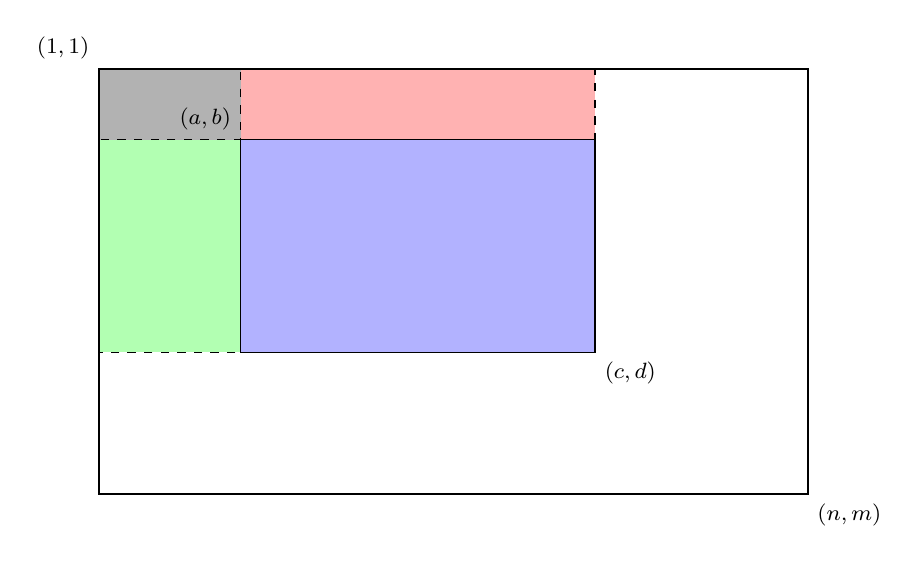
\begin{tikzpicture}[scale=0.9]
            \draw[dashed,fill=red!30] (0, 5) rectangle (7, 6);
            \draw[dashed,fill=green!30] (0, 2) rectangle (2, 6);
            \draw[dashed,fill=black!30] (0, 5) rectangle (2, 6);
            \draw[fill=blue!30] (2, 2) rectangle (7, 5);
            \draw[thick] (0, 0) rectangle (10, 6);

            \node[anchor=north west] at (7, 2) { \footnotesize $(c, d)$ };
            \node[anchor=south east] at (2, 5) { \footnotesize $(a, b)$ };
            \node[anchor=south east] at (0, 6) { \footnotesize $(1, 1)$ };
            \node[anchor=north west] at (10, 0) { \footnotesize $(n, m)$ };
        \end{tikzpicture}
    \end{figure}

\end{frame}


\begin{frame}[fragile]{Max 2D Range Sum PD}
    \inputsnippet{cpp}{7}{27}{codes/max-2D-range-sum_dp.cpp}
\end{frame}
